%!TEX root = main.tex
\newpage
\chapter{Návrh riešenia personalizovaného informačného bulletinu v CQA systéme}

Cieľom našej práce je navrhnúť, zrealizovať a overiť metódu zostavovania personalizovaných informačných bulletinov v CQA systémoch
so zameraním sa na podporu diverzity a~aktuálnosti obsahu odporúčaného v informačnom bulletine.

Naše riešenie je navrhnuté pre použitie vrámci platformy Stack Exchange, ktorá patrí medzi najpopulárnejšie CQA systémy
v súčasnosti a tvorí ju viac ako 160 komunít zameraných na rôzne oblasti.

Informačný bulletin bude tvoriť viacero sekcií, ktoré vyžadujú rôzne spôsoby odporúčania. Konkrétne ide o odporúčanie
nových otázok a odporúčanie vyriešených otázok, pričom v prvom prípade je dôležité pozerať sa na expertízu používateľa
a v druhom prípade na oblasti jeho záujmu.

\textbf{Hypotéza 1}\\
\textit{Použitím personalizovaného odporúčania otázok v informačnom bulletine CQA systému zvýšime relevanciu obsahu informačného
bulletinu, čo sa prejaví zvýšenou mierou jeho používania medzi používateľmi CQA systému.}

\textbf{Hypotéza 2}\\
\textit{Výberom odporúčaných otázok zo širšieho okruhu záujmu používateľa a zohľadnením ich aktuálnosti predídeme výskytu problému
filtračnej bubliny, čím dosiahneme vyššiu mieru záujmu používateľa a jeho aktivity.}

\textbf{Prehľad navrhovanej metódy}\\
Na začiatok uvádzame stručný súhrn navrhnutej metódy zostavovania personalizovaných informačných bulletinov.
Celkový pohľad na metódu ilustruje obrázok~\ref{fig:overview}, Jednotlivé časti metódy sú podrobne opísané v nasledujúcich kapitolách.
\begin{my_itemize}
\item{
    Pre zostavenie personalizovaných informačných bulletinov využijeme odporúčaciu metódu filtrovania na základe obsahu
    (kap.~\ref{rec:content}), keďže je v prípade malej používateľskej aktivity efektívnejšia ako kolaboratívne filtrovanie
    (viď kap.~\ref{cold-start}).
}
\item{
    Diverzifikáciu odporúčaného obsahu budeme zabezpečovať na úrovni tématického pre-filteru pred samotným procesom
    odporúčania -- pre každú nezávislú tému sa bude vytvárať samostatný zoznam odporúčaní.
    Pri návrhu tejto metódy sme sa vychádzali z~\cite{Szpektor2013}.
}
\item{Výsledný zoznam odporúčaného obsahu vznikne spojením jednotlivých zoznamov z kroku diverzifikácie.}
\item{Pri odporúčaní sa okrem diverznosti a relevancie obsahu bude uvažovať aj jeho aktuálnosť.}
\end{my_itemize}

\textbf{TODO - sem pojde flow diagram znazorujuci cely proces zostavovania odporucani}\label{fig:overview}

\section{Návrh metódy personalizovaného odporúčania}


Pri vytváraní personalizovaného informačného bulletinu sa budeme zameriavať na odporúčanie relevantných otázok jednotlivým
používateľom CQA systému prostredníctvom aplikovania metódy filtrovania na základe obsahu (kapitola~\ref{rec:content}).
Pre účely filtrovania na základe obsahu je potrebné definovať a zostaviť modely reprezentujúce jednak otázky, a tiež
používateľov CQA systému.

\subsection{Model otázok}

Model otázky sa bude skladať z troch nezávislých modelov, ktoré sa na samotnú otázku pozerajú z rôznych perspektív.

\textbf{1. Kategorický model otázok}\\
Tento model reprezentuje otázku na najvyššej úrovni ako prislúchajúcu do určitých kategórií. Kategórie otázok sú vrámci
platformy Stack Exchange reprezentované ako značky (angl.~\textit{tags}). Každá otázka môže obsahovať viacero značiek.

Samotný kategorický model otázky bude reprezentovaný ako vektor v $n$-rozmernom priestore, kde každý rozmer $n_i$
predstavuje príslušnosť otázky k danej značke. Nakoľko značky netvoria hierarchickú štruktúru, bude vektor v jednotlivých
rozmeroch nadobúdať iba hodnoty $0$~alebo~$1$.

\textbf{2. Tématický model otázok}\\
Tématický model využíva metódu latentnej Dirichletovej alokácie (angl.~\emph{Latent Dirichlet Allocation - LDA})~\cite{blei2003latent}
na určenie latentnej témy, ktorej sa daná otázka venuje.

LDA vektor tohto modelu bude reprezentovať distribúciu otázky vrámci jednotlivých latentných tém.
Samotné LDA témy sa budú odvodzovať z nadpisu a textu otázky.
Pre optimalizáciu modelu a zanedbanie tém s veľmi nízkou distribúciou sa do úvahy budú brať len latentné témy tvoriace
75\% z celkovej distribúcie, teda tretí kvartil. Jednotlivé hodnoty tém budú následne normalizované, aby tvorili 100\%.

\begin{figure}[H]\begin{center}
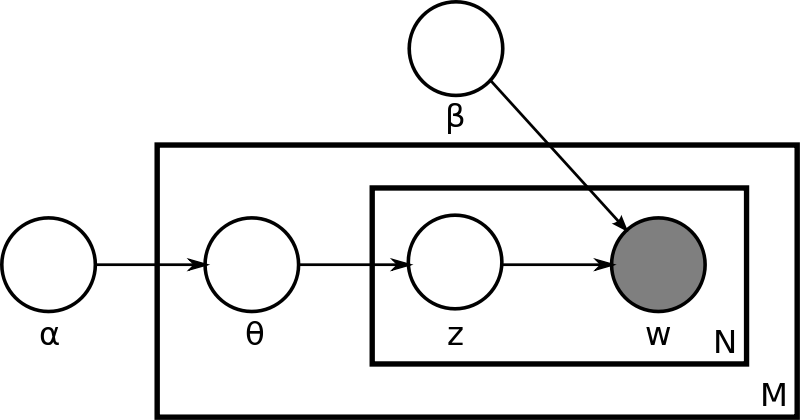
\includegraphics[scale=0.3]{lda-plate}
\caption{Platňová notácia LDA modelu.\footnotemark}\end{center}
\end{figure}
\footnotetext{Prevzaté 10.12.2017 z \url{https://en.wikipedia.org/wiki/Latent_Dirichlet_allocation}}

\begin{adjustwidth}{1cm}{1cm}
\textbf{Nastavenie LDA}\\
Pre určenie vhodného počtu LDA tém ($n$) využijeme metódu hierarchických Dirichletových procesov~\cite{Teh2006}.
Pre trénovanie LDA modelu bude využitý online variačný Bayesov algoritmus. Parametre modelu budú nastavené nasledovne:\\
$$\alpha = \frac{1}{n}; \kappa = 0.7; \tau_0 = 10; \eta = \frac{1}{n}$$

$M$ -- Celkový počet dokumentov. \\
$N$ -- Celkový počet slov vo všetkých dokumentoch. \\
$Z$ -- $N$-rozmerný vektor identít tém všetkých slov vo všetkých dokumentoch. \\
$W$ -- $N$-rozmerný vektor identít všetkých slov vo všetkých dokumentoch. \\
$n$ -- Celkový počet tém. \\
$\alpha$   -- Úvodná váha tém v dokumente. $1/n$ zabezpečí v úvode rovnomernú distribúciu.\\
$\beta$    -- Úvodná váha slov v téme. $1/n$ zabezpečí v úvode rovnomernú distribúciu.\\
$\theta_d$ -- Distribúcia tém v dokumente $d$. \\
$\kappa$   -- Úpadok učenia; parameter kontrolujúci mieru učenia v online metóde učenia. \\
$\tau_0$   -- Posun učenia; znižuje váhu počiatočným iteráciám v online metóde učenia.

Nakoľko jednotlivé komunity vrámci platformy Stack Exchange sú pomerne úzko zamerané, predpokladáme, že bude dostačujúce
natrénovať LDA model na vzorke archívnych dát a nebude potrebné postupné dotrénovanie modelu. Napriek tomu sme zvolili
online variačný Bayesov algoritmus, keďže je pri veľkom množstve dát efektívnejší ako dávková varianta tohto algoritmu.
\end{adjustwidth}

\textbf{3. Lexikálny model otázok}\\
Lexikálny model otázky využíva TF-IDF vektor reprezentujúci zastúpenie jednotlivých výrazov v texte otázky. Rovnako ako
LDA vektor bude zostavený z nadpisu a textu samotnej otázky. Pred výpočtom bude text lematizovaný a budú z neho odstránené
stop slová.

$$\textrm{tf-idf}(t, d) = \textrm{tf}(t, d) \times \log\frac{n_d}{1+\textrm{df}(d, t)}$$

\subsection{Model používateľov}

Pre každého používateľa budeme uvažovať dva nezávislé modely -- jeden bude modelovať záujem používateľa o určité témy a otázky,
druhý bude modelovať jeho expertízu v určitej oblasti. Jeden bude použitý
pri odporúčaní otázok, ktoré by používateľa mohli zaujímať, druhý pri odporúčaní otázok, ktoré by mohol vedieť zodpovedať.
Oba modely budú z pohľadu svojej štruktúry presne rovnaké.

Takýto prístup k rozdeleniu modelu používateľa podľa záujmu a expertízy je vo svojej podstate unikátny, nakoľko ho využíva
iba práca~\cite{Xu2012}. V ostatný prácach autori buď modelujú len jeden z týchto aspektov, alebo ich vôbec nerozlišujú~\cite{Srba2016}.

Model používateľa bude zostavený na základe jeho aktivity a bude sa analogicky k modelu otázok skladať z troch vektorov:

\begin{my_enumerate}
\item{
  Prvý vektor bude reprezentovať aktivitu používateľa naprieč značkami -- každý rozmer bude predstavovať jednu značku,
  v ktorej má používateľ aktivitu. Hodnoty v jednotlivých rozmeroch budú predstavovať podiel aktivity v danej značke voči
  celkovému množstvu aktivity používateľa.
}
\item{
  Druhý vektor bude analogicky k prvému reprezentovať aktivitu používateľa naprieč LDA témami, v ktorých má používateľ aktivitu.
}
\item{
  Tretí vektor bude reprezentovať zastúpenie jednotlivých výrazov v textoch otázok, v ktorých má používateľ aktivitu.
}
\end{my_enumerate}

\textbf{Záujmový model}\\
Model predstavujúci záujem používateľa bude zostavený zo všetkých otázok, ktoré používateľ položil, alebo ktoré označil
za obľúbené. Každá takáto otázka bude do modelu prispievať rovnakou váhou.

\textbf{Expertízny model}\\
Model modelujúci expertízu používateľa sa bude skladať z otázok, na ktoré používateľ odpovedal, pričom ich dopad na model
expertízy bude závislý od skóre jeho odpovede. Kladné skóre bude prisipevať do modelu pozitívne -- bude to teda signalizovať
fakt, že používateľ danej téme rozumie. Odpoveď so záporným skóre bude naopak signalizovať, že používateľ danej téme nerozumie,
čo bude reflektované aj v jeho expertíznom modeli. Odpovede označené za akceptované budú do modelu prispievať
s~koeficientom, ktorého hodnota bola empiricky stanovená na $1.5$.

\textbf{Komentáre}\\
Okrem pokladania otázok, odpovedania alebo označenia za obľúbené budú uvažované aj používateľove komentáre. Keďže však
zo samotného faktu že používateľ niečo okomentoval nemožno jednoznačne určiť, či táto aktivita predstavuje jeho záujem
alebo expertízu, budú otázky, ktoré používateľ okomentoval prispievať do oboch modelov -- záujmového aj expertízneho, avšak
s~koeficientom, ktorého hodnota bola empiricky stanovená na $\frac{1}{3}$.

\subsection{Výber odporúčaného obsahu}\label{design:rec-retrieval}

Pre účely zostavovania zoznamu odporúčaných otázok použijeme prístup analogický štandardným nástrojom pre vyhľadávanie
informácií (angl.~\emph{Information Retrieval Engines}). V našom prípade budú dokumentmi samotné otázky a dopytom bude
model používateľa. Pre ohodnocovanie podobnosti modelov bude použitý skalárny súčin vektorov reprezentujúcich
modely otázky a používateľa.

\textbf{Skalárny súčin (angl.~\textit{dot product}) vektorov $\mathbf{a}$ a $\mathbf{b}$.}\\
$$\mathbf{a}\cdot\mathbf{b}=\sum_{i=1}^n a_ib_i=a_1b_1+a_2b_2+\cdots+a_nb_n$$

\subsection{Riešenie problému studeného štartu}

Pre eliminovanie problému studeného štartu (kapitola~\ref{cold-start}) z pohľadu prvotného odporúčania otázok využijeme
offline natrénovanie našich metód na archívnych dátach platformy Stack~Exchange.

V prípade nových používateľov, ktorí v systéme nemajú žiadnu, alebo iba nedostatočnú aktivitu, budeme zo začiatku vytvárať
iba generický informačný bulletin podobný tomu, ktorý je používateľom k dispozícii aj v súčasnosti (kapitola~\ref{so-newsletter}).


\subsection{Aktuálnosť odporúčaní}

Pri zostavovaní odporúčaní do informačného bulletinu sa budú uvažovať len otázky, ktoré pochádzajú
z obdobia od posledného zostavenia informačného bulletinu.

Aby model používateľa reflektoval meniace sa záujmy používateľa v čase, zavedieme pri zostavovaní modelu z používateľovej
aktivity exponenciálny \textit{faktor úpadku} (angl.~\textit{decay factor}):
$$y_{n+t} = y_n (1 - d)^t$$

\begin{adjustwidth}{1cm}{1cm}
$y_n$ -- aktuálna váha danej veličiny v modeli používateľa\\
$y_{n+t}$ -- váha danej veličiny po aplikovaní faktoru úpadku\\
$t$ -- čas od pregenerovania modelu používateľa -- počet pregenerovaní modelu.\\
$d$ -- percentuálny pokles danej veličiny; vypočíta sa ako podiel množstva používateľovej aktivity za čas $t$ a jeho celkového množstva aktivity.
\end{adjustwidth}

\section{Návrh metód diverzifikácie odporúčaní}

Diverzifikácia obsahu personalizovaného informačného bulletinu sa bude vykonávať ešte pred samotným zostavovaním
zoznamu odporúčaní formou pre-filteru. Diverzifikácia bude spočívať vo výbere \textit{značiek} a \textit{tém}, pričom
následne v kroku zostavovania zoznamov odporúčaní sa bude pre každý zoznam uvažovať len obsah prislúchajúci do danej
značky alebo témy. Okrem výberu značiek a tém bude diverzifikácia aplikovaná aj pri následnom výbere položiek z jednotlivých
zoznamov do výsledného zoznamu odporúčaní.

Tento prístup k diverzifikácii sme zvolili okrem jeho prirodzenosti aj z dôvodu jeho veľmi dobrej škálovateľnosti,
nakoľko alternatívny prístup postavený na tvorbe odporúčaní nad všetkým obsahom daného CQA systému a až následnej
diverzifikácií by v praxi nebol realizovateľný. Ako príklad môžeme uviesť systém Stack Overflow, kde denne pribudne
cca 8-9000 nových otázok, čo by v prípade generovania týždenného informačného bulletinu znamenalo vypočítať podobnosť
až cca 60000 modelov otázok s modelom každého používateľa.

Cieľom našej práce je vyhodnotiť dopad diverzifikácie odporúčaní na personalizované informačné bulletiny CQA systémov.
Za týmto účelom sme navrhli dve metódy diverzifikácie odporúčaní: metódu proporčnej diverzifikácie a metódu tématického vzorkovania.

\subsection{Metóda proporčnej diverzifikácie}

Zostavenie výsledného zoznamu $n$ odporúčaní s použitím metódy proporčnej diverzifikácie je navrhnuté nasledovne:

\begin{my_enumerate}
\item{
    Pre každého používateľa vyberieme z jeho záujmového alebo expertízneho modelu $k$~najvyššie hodnotených značiek
    z~kategorického vektoru a $k$~najvyššie hodnotených tém z~tématického vektoru, pričom
    $2 \times k = \left\lceil\frac{n}{2}\right\rceil$.
}
\item{
    Prostredníctvom vyššie opísanej metódy (kapitola~\ref{design:rec-retrieval}) sa pre každú takúto značku a tému
    následne zostaví zoznam $n$ odporúčaní, pričom sa budú uvažovať len otázky prislúchajúce tejto téme alebo značke.
}
\item{
    Následne sa z každého zoznamu vyberie vrchných $n_k$ odporúčaných položiek, pričom $n_k = \frac{n}{2k}$
}
\end{my_enumerate}

Metóda proporčnej diverzifikácie tak v podstate používateľovi vyberie najrelevantnejšie položky z jeho najrelevantnejších
tém a značiek. Túto jednoduchú metódu diverzifikácie budeme následne porovnávať s metódou tématického vzorkovania.


\subsection{Metóda tématického vzorkovania}

Pri návrhu tejto metódy sme sa inšpirovali rovnomennou metódou z~\cite{Szpektor2013}, ktorú sme prispôsobili
podmienkam špecifickým pre našu prácu. Proces tématického vzorkovania ilustruje schéma na obrázku~\ref{fig:tematic-sampling}.

\begin{my_enumerate}
\item{
    Pre každého používateľa vyberieme z jeho modelu $k_1$~značiek a~$k_2$~tém. Pri výbere sa obmedzíme na značky a témy,
    ktoré spadajú do druhého kvartilu -- mediánu. Potlačíme tak značky a témy, ktoré majú pre používateľa nízku relevanciu.\\
    $k_1 + k_2 = \left\lceil\frac{n}{2}\right\rceil$; konkrétne hodnoty pre $k_1$ a $k_2$ nešpecifikujeme, $n$ je počet
    odporúčaní vo~výslednom zozname.
}
\item{
    Prostredníctvom vyššie opísanej metódy (kapitola~\ref{design:rec-retrieval}) sa pre každú takúto značku a tému
    následne zostaví zoznam $n$ odporúčaní, pričom sa budú uvažovať len otázky prislúchajúce tejto téme alebo značke.
}
\item{
    Následne budeme náhodne vyberať vzorky z jednotlivých zoznamov do výsledného zoznamu odporúčaní, pričom pravdepodobnosť
    výberu otázky z konkrétneho zoznamu $P_s(l_i)$ bude proporčná k relevancii tejto témy pre daného používateľa.
}
\item{
    Konkrétne otázky z jednotlivých zoznamov sa budú vyberať z~$m = P_s(l_i)$ najrelevantnejších otázok daného zoznamu
    v náhodnom poradí.

}
\end{my_enumerate}

\begin{figure}[H]\begin{center}
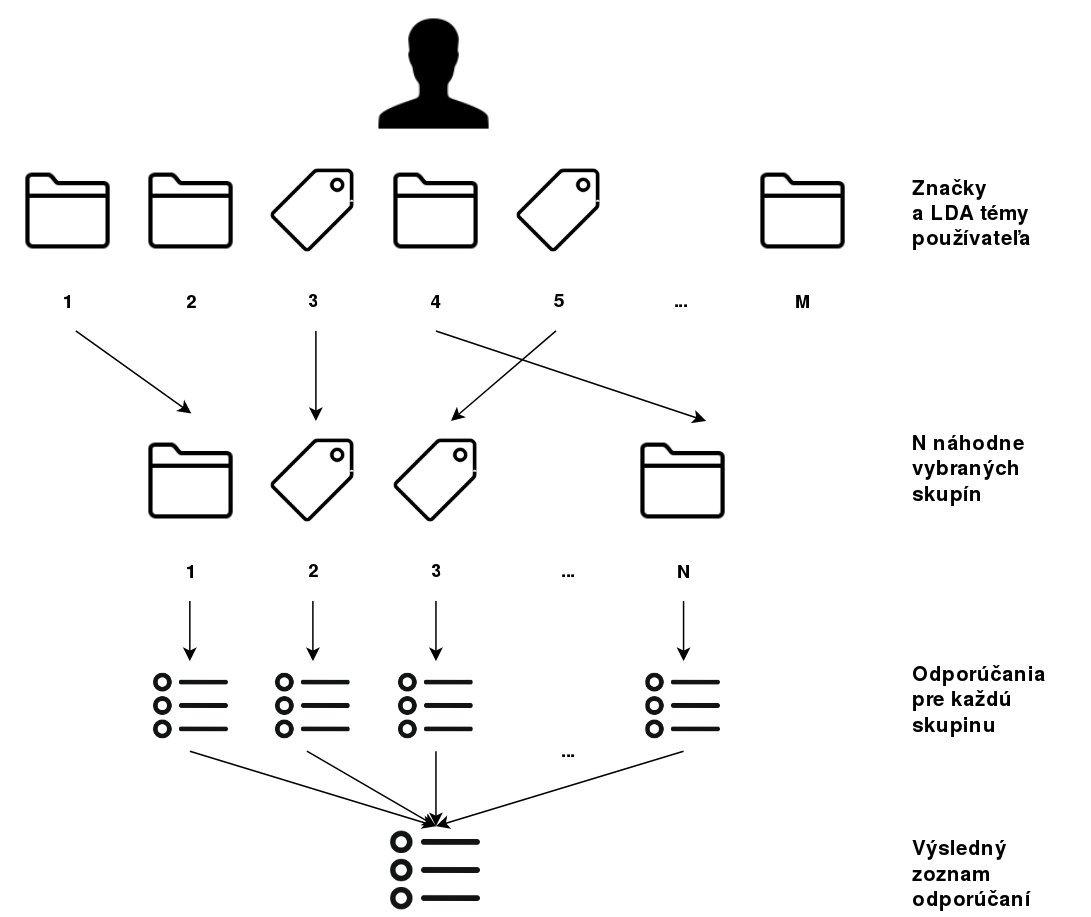
\includegraphics[scale=0.27]{diversity-diagram}
\caption{Schéma metódy diverzifikácie odporúčaní tématickým vzorkovaním.\label{fig:tematic-sampling}}\end{center}
\end{figure}


\section{Metriky hodnotenia výsledkov}

Pre overovanie výsledkov experimentov budeme používať tieto metriky:

\textbf{Precision@N}\\
Presnosť (angl.~\emph{Precision}), alebo tiež \textit{pozitívna predikčná hodnota} je metrika reprezentujúca pomer relevantných
dokumentov z celkového zoznamu. Štandardne sa presnosť počíta ako pomer z celého zoznamu dokumentov, no v oblasti
odporúčania a vyhľadávania informácií je často vhodnejšou odvodená metrika \textit{Precision@N}, ktorá určuje, aká časť
z prvých N dokumentov v zozname je relevantná.
$$\mbox{Precision@N}=\frac{|\{\mbox{relevantne otazky v top-N}\}\cap\{\mbox{top-N odporucenych otazok}\}|}{|\{\mbox{top-N odporucenych otazok}\}|}$$

\textbf{nDCG}\\
\textit{Normalized Discounted Cumulative Gain} je metrika kvality ohodnocovania často používaná na meranie efektívnosti
odporúčania. DCG meria užitočnosť dokumentov na základe ich pozície vo výslednom zozname. Užitočnosť dokumentov sa akumuluje
od konca zoznamu, pričom najvyššiu užitočnosť majú dokumenty na začiatku zoznamu~\cite{Jrvelin2002}.

nDCG položky na pozícii $p$ v zozname odporúčaní je definované ako:

$$\mathrm{nDCG_{p}} = \frac{DCG_{p}}{IDCG_{p}}$$
$$\mathrm{DCG_{p}} = \sum_{i=1}^{p} \frac{ 2^{rel_{i}} - 1 }{ \log_{2}(i+1)}$$
$$\mathrm{IDCG_{p}} = \sum_{i=1}^{|REL|} \frac{ 2^{rel_{i}} - 1 }{ \log_{2}(i+1)}$$
\begin{adjustwidth}{1cm}{1cm}
$rel_i$ -- relevancia $i$-tej položky v zozname odporúčaní.\\
$|REL|$ -- zoznam $p$ relevantných položiek zo zoznamu odporúčaní usporiadaných podľa relevancie.
\end{adjustwidth}

\textbf{CTR}\\
Miera preklikov (angl.~\emph{Click-through Rate}) je metrika často využívaná v spojitosti s informačnými bulletinmi.
Táto metrika vyjadruje počet úspešných kliknutí na odkaz v informačnom bulletine.

Okrem CTR plánujeme v súvislosti s interakciou používateľa s informačným bulletinom merať aj počet impresií,
teda zobrazení informačného bulletinu, ako aj počet konverzií, teda podiel prípadov, kedy kliknutie na niektorú z otázok
v informačnom bulletine viedlo k aktivite používateľa na tejto otázke -- či už označenie za obľúbenú,
odpovedanie alebo pridanie komentáru. Ďalej tiež plánujeme merať počet odhlásení z informačného bulletinu.


\section{Návrh overenia metód}

Nami navrhnuté metódy personalizovaného odporúčania a diverzifikácie odporúčaného obsahu budeme overovať prostredníctvom
online nekontrolovaného experimentu spoločne s kolegom Matúšom Salátom~\cite{Salat2018} na používateľoch z komunity \textit{Stack Overflow} platformy Stack Exchange.

Tento online experiment bude mať formu pravidelne rozposielaného informačného bulletinu, na ktorého odoberanie sa budú
môcť prihlásiť všetci používatelia z tejto komunity.

Účinnosť zvolených metód diverzifikácie odporúčaní budeme vyhodnocovať prostredníctvom A/B testovania, pričom používateľov
rozdelíme na štyri skupiny:
\begin{my_enumerate}
    \item{Kontrolná skupina -- generický informačný bulletin bez odporúčania;}
    \item{Skupina A -- informačný bulletin s odporúčaním, bez diverzifikácie;}
    \item{Skupina B -- informačný bulletin s odporúčaním, metóda proporčnej diverzifikácie;}
    \item{Skupina C -- informačný bulletin s odporúčaním, metóda tématického vzorkovania;}
\end{my_enumerate}

Dôležitým predpokladom pre úspešnosť online experimentu bude získať dostatočnú reprezentatívnu vzorku používateľov
ochotných byť súčasťou experimentu. V~prípade, že by sa nám nepodarilo osloviť dostatočný počet používateľov, plánujeme
vykonať kontrolovaný offline experiment na vzorke archívnych dát.


